This chapter gives a short representation of the first platform design and the chosen technologies and frameworks. First, the Ethereum blockchain is implemented through Ganache. It is a personal local blockchain for the Ethereum development, which can be used to deploy smart contracts, develop decentralized applications, and run tests. Further, Ganache is available as a desktop application as well as a command-line tool. Next, the role of the market dealer is realized by a smart contract which is written in Solidity. This object-oriented programming language was especially designed for developing smart contracts that run on a Ethereum blockchain. The Solidity code is compiled to bytecode, which can be deployed into the blockchain. Moreover, the clients which constitute the different agents are implemented through the programming language Python. Python is a object oriented, high-level programming  language with a easy and simple to learn syntax. Therefore, the hurdles in modifying the client behavior are minimized. Finally, the clients using the Web3.py python library for the interaction with the Ethereum blockchain. 

\begin{figure}[htbp]
	\centering
	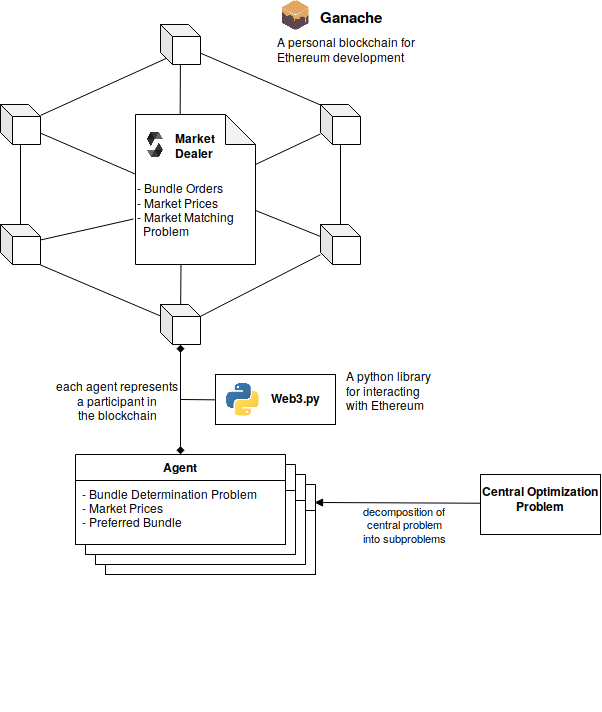
\includegraphics[width=.8\linewidth]{./figures/platform_architecture.png}
	\caption{Platform Design}
	\label{figure:paltform_architecture}
\end{figure}